\chapter{Long Polling}
\label{chap:long_polling}
In questo capitolo si spiega il funzionamento del modello di comunicazione 
Long Polling, per poi spiegare come è applicato in unicam-product-editor, 
ed infine compararlo con altre metologie in uso.

L'XMLHTTPRequest Long Polling è, di base, una tecnologia dove il client 
richiede un'informazione al server senza aspettarsi una risposta immediata.
Questo fa sì che la connessione che esiste fra client e server abbia una 
connessione di lunga durata, durante la quale il server esegue un'operazione 
complessa, e solo una volta portata a termine, restituisce una risposta al 
client inviando i dati richiesti come risposta, o anche solo una notifica.

Innanzitutto il fatto che questa tecnologia sia basata su XMLHTTPRequest 
ci fa capire che le chiamate che il client effettua nei confronti del 
server sono delle semplici chiamate Ajax, ma a differenza dell'uso 
tradizionale di queste chiamate, la gestione degli eventi non viene 
eseguita dalla parte del client (client-side), ma dalla parte del 
server (server-side).Inoltre, a differenza delle chiamate Ajax, che 
vengono effettuate a intervalli regolari, ad esempio ogni 10 secondi 
al termine delle quali la connessione al server viene chiusa, in una 
chiamata di tipo Long Polling, la connessione col server rimane aperta 
finché il server stesso non invia una risposta, oppure finché non si 
raggiunge un limite di tempo impostato, detto timeout.

Questo tipo di tecnlogia usato nelle applicazioni non è nuovo, le web 
chat sono sempre esistite. Quello che è cambiato negli ultimi anni è 
l’approccio tecnologico a basso livello. Una volta i client facevano 
richieste HTTP ogni pochi secondi al server richiedendo eventuali 
messaggi (come ad esempio nel protocollo POP3 per la ricezione delle 
email) mentre nel Long Polling è il server stesso a notificare il 
client solamente a fronte di novità.
\newpage
Di seguito uno schema che riassume l'architettura Long Polling, 
mostrando l'interazione fra un client e un server, e le relative 
richieste e risposte.
\begin{figure}[h]
	\centering
	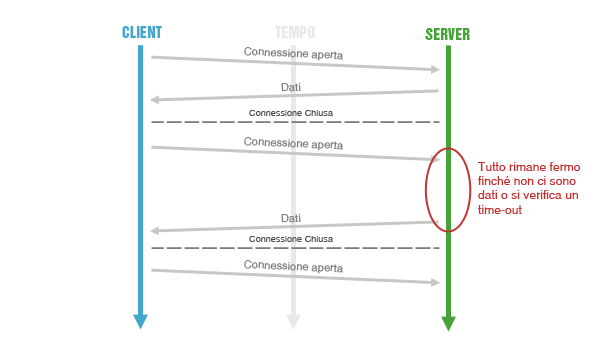
\includegraphics[scale=0.7]{Immagini/long_polling.png}
	\caption{Modello di comunicazione Long Polling}
\end{figure}

Questo metodo, assieme ad altri con lo stesso funzionamento di base 
(ad esempio lo Streaming) insieme costituiscono il modello architetturale 
Comet, in cui le richieste HTTP di lunga durata che permettono ad un web 
server di inviare dati ad un browser senza che quest'ultimo li abbia 
esplicitamente richiesti ne sono la caratteristica principale.

La tecnica del Long Polling, nonostante non sia difficilissima da 
implementare una volta compresa, non può essere però eseguita in 
qualsiasi server web proprio per la caratteristica di avere richieste 
in stato “pending”. I principali server web e application server non 
offrono questa funzionalità nativa perchè agiscono, differentemente da 
Node.js, in maniera sincrona. Hanno a disposizione un numero finito di 
“slot di richieste”, esaurito il quale sono obbligati a rilasciarne qualcuna.
NodeJS grazie al suo modello \emph{event-driven} offre una struttura di 
basso livello che eccelle in questo tipo di applicazioni. Il meccanismo 
basato su callback rappresenta il deux ex machina per un architettura 
basata su Long Polling.

In unicam-product-editor, e più precisamente nella fase di upload di 
un oggetto 3D, il caso base che si verificherà sarà quello del client 
che inizia il caricamento della forma attraverso l'interfaccia, 
inviando una richiesta HTTP al server Node.js, il quale inizierà in 
sequenza le fasi di upload, conversione in JSON e inserimento del file 
convertito nel database. Durante questo processo, che per sua natura 
ha un tempo di esecuzione lungo (essendo i file 3D in formato .obj ed 
i corrispondenti file JSON una dimensione media nell'ordine dei MegaByte) 
la richiesta HTTP rimane in una fase di congelamento, finché il server 
non avrà eseguito tutto il processo, ed invierà al client una risposta 
(sia essa di successo nell'esecuzione o di errore), o finché non si 
sarà raggiunto il tempo limite, detto timeout, superato il quale la 
richiesta si esaurirà.

Il Long Polling HTTP inoltre è utilissimo per creare API affidabili, 
in quanto le azioni di sincronizzazione e di ascolto possono essere 
combinate in una stessa richiesta. Nel nostro caso, essendo questo 
progetto basato su RESTful API, è facile espandere una di queste 
trasformandola in una Long Polling API, mantenendo comunque la stessa 
semantica, usando anche questo sistema delle interazioni di tipo 
\emph{request/response}. Dei timeout brevi possono oltretutto aumentare 
la solidità delle richieste fra client e server nel caso in cui, ad 
esempio, l'indirizzo IP di un client cambi come conseguenza del roaming 
da rete wireless a rete mobile o tethering.

E' per questi motivi che in unicam-product-editor è stata implementata 
la tecnologia di Long Polling nella fase di upload di una forma 3D.
Il tutto rende il processo di upload non bloccante, ossia permette 
all'utente, durante l'esecuzione delle operazioni sopra elencate, di 
continuare ad eseguire altre operazioni sulla applicazione web, mentre 
il processo viene portato a termine in background.
Per rendere ciò possibile, dobbiamo ricordarci che il progetto è basato 
su un server Node.js, il quale è di tipo \emph{event-driven}, ed esegue 
le operazioni in modo asincrono. Proprio per questa caratteristica, 
la fase di upload di un oggetto 3D non è bloccante nei confronti 
dell'utente, che può così continuare ad inviare al server normali 
richieste HTTP.

\section{Implementazione del Long Polling in unicam-product-editor}
In questa fase andremo a vedere l'uso pratico della tecnologia appena 
descritta nel nostro editor di forme 3D.

Per quanto riguarda le normali chiamate HTTP Ajax, è stata usata 
jQuery\cite{jquery}, una libreria JavaScript veloce, leggera e 
ricca di funzionalità.

Prendiamo in esame il Controller Angular su cui si sviluppa la 
pagina dell'uploader:

\begin{lstlisting}[{caption=HTTP POST /upload}, style=JavaScriptCode]
$http.post('/upload', fd, {
	withCredentials: true,
	headers: {'Content-Type': undefined },
	transformRequest: angular.identity
})
\end{lstlisting}
Per prima cosa si esegue la HTTP POST request relativa all'upload e 
successiva conversione del file .obj. La chiamata API è indicata 
subito dopo la funzione \texttt{\$http.post}, ed è \texttt{/upload}.
La risposta che arriverà da parte del server sarà l'endpoint del 
file JSON convertito, che metteremo nella variabile \texttt{filename}.
Dopo questo si esegue una chiamata HTTP GET, passando come parametro 
il nome del file appena convertito, per inserire il file JSON nel database.  

\begin{lstlisting}[{caption=HTTP GET /insert}, style=JavaScriptCode]
$http({method: 'GET', url: filename})
	.then(function successGet(filename) {
		$http({method: 'POST',
			url: '/insert',
			data: {shape: filename.data}
		})
	...
\end{lstlisting}

La gestione degli errori avviene tramite la funzione \texttt{.then} 
della richiesta HTTP: se l'operazione va a buon fine, la risposta 
del server sarà il codice \texttt{200, OK}, mentre in caso 
contrario il server risponderà con un codice di errore. In entrambi 
i casi il risultato è contenuto nel parametro \texttt{response}.

\begin{lstlisting}[{caption=gestione degli errori nella richiesta HTTP}, style=JavaScriptCode]
.then(function successResponse(response){
	console.log(response);
	console.log('file inserted in db');
	$scope.isRouteLoading = false;
	$scope.uploadsuccess = true;
}, function errorResponse(response) {
	console.log(response);
	console.log('error in insert');
});
\end{lstlisting}

\section{Altri metodi di comunicazione fra client e server}
Di seguito vengono elencati, oltre al Long Polling, gli altri 
metodi di comunicazione fra client e server, con particolare 
riguardo al modo in cui vengono scambiate le richieste fra i 
due interlocutori.

\subsection{Normale HTTP}
\begin{enumerate}
	\item Il client richiede una pagina web al server.
	\item Il server calcola la risposta.
	\item Il server invia la risposta al client.
\end{enumerate}
\begin{figure}[h]
	\centering
	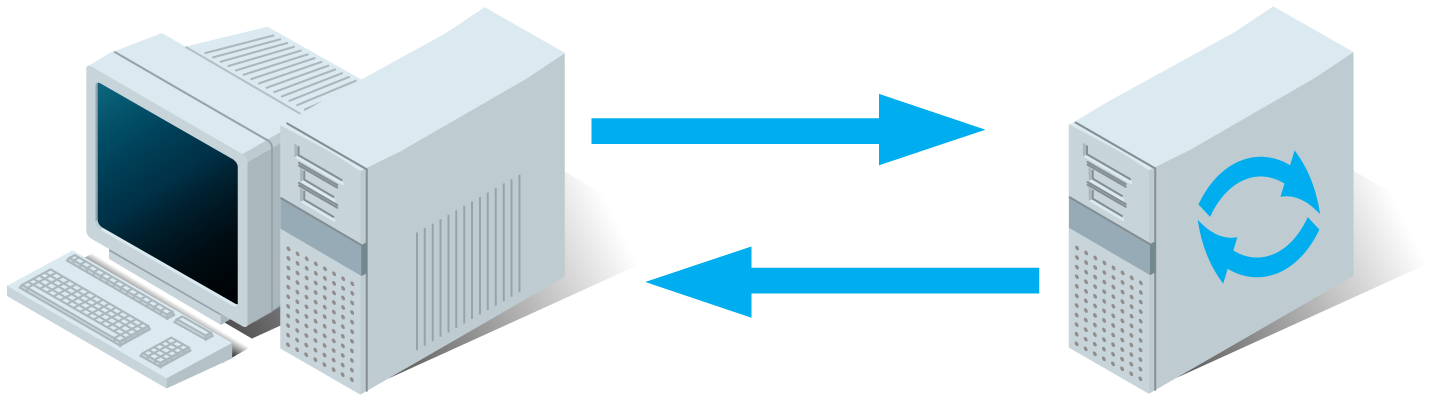
\includegraphics[scale=0.4]{Immagini/regular_http.png}
\end{figure}
\subsection{Polling Ajax}
\begin{enumerate}
	\item Il client richiede una pagina web al server usando  il normale HTTP.
	\item Il client riceve la pagina web richiesta ed esegue il codice JavaScript contenuto nella pagina, il quale richiede un file al server ad intervalli regolari (es. 0.5 secondi).
	\item Il server calcola ogni risposta e la invia al client, come del normale traffico HTTP.
\end{enumerate}
\begin{figure}[h]
	\centering
	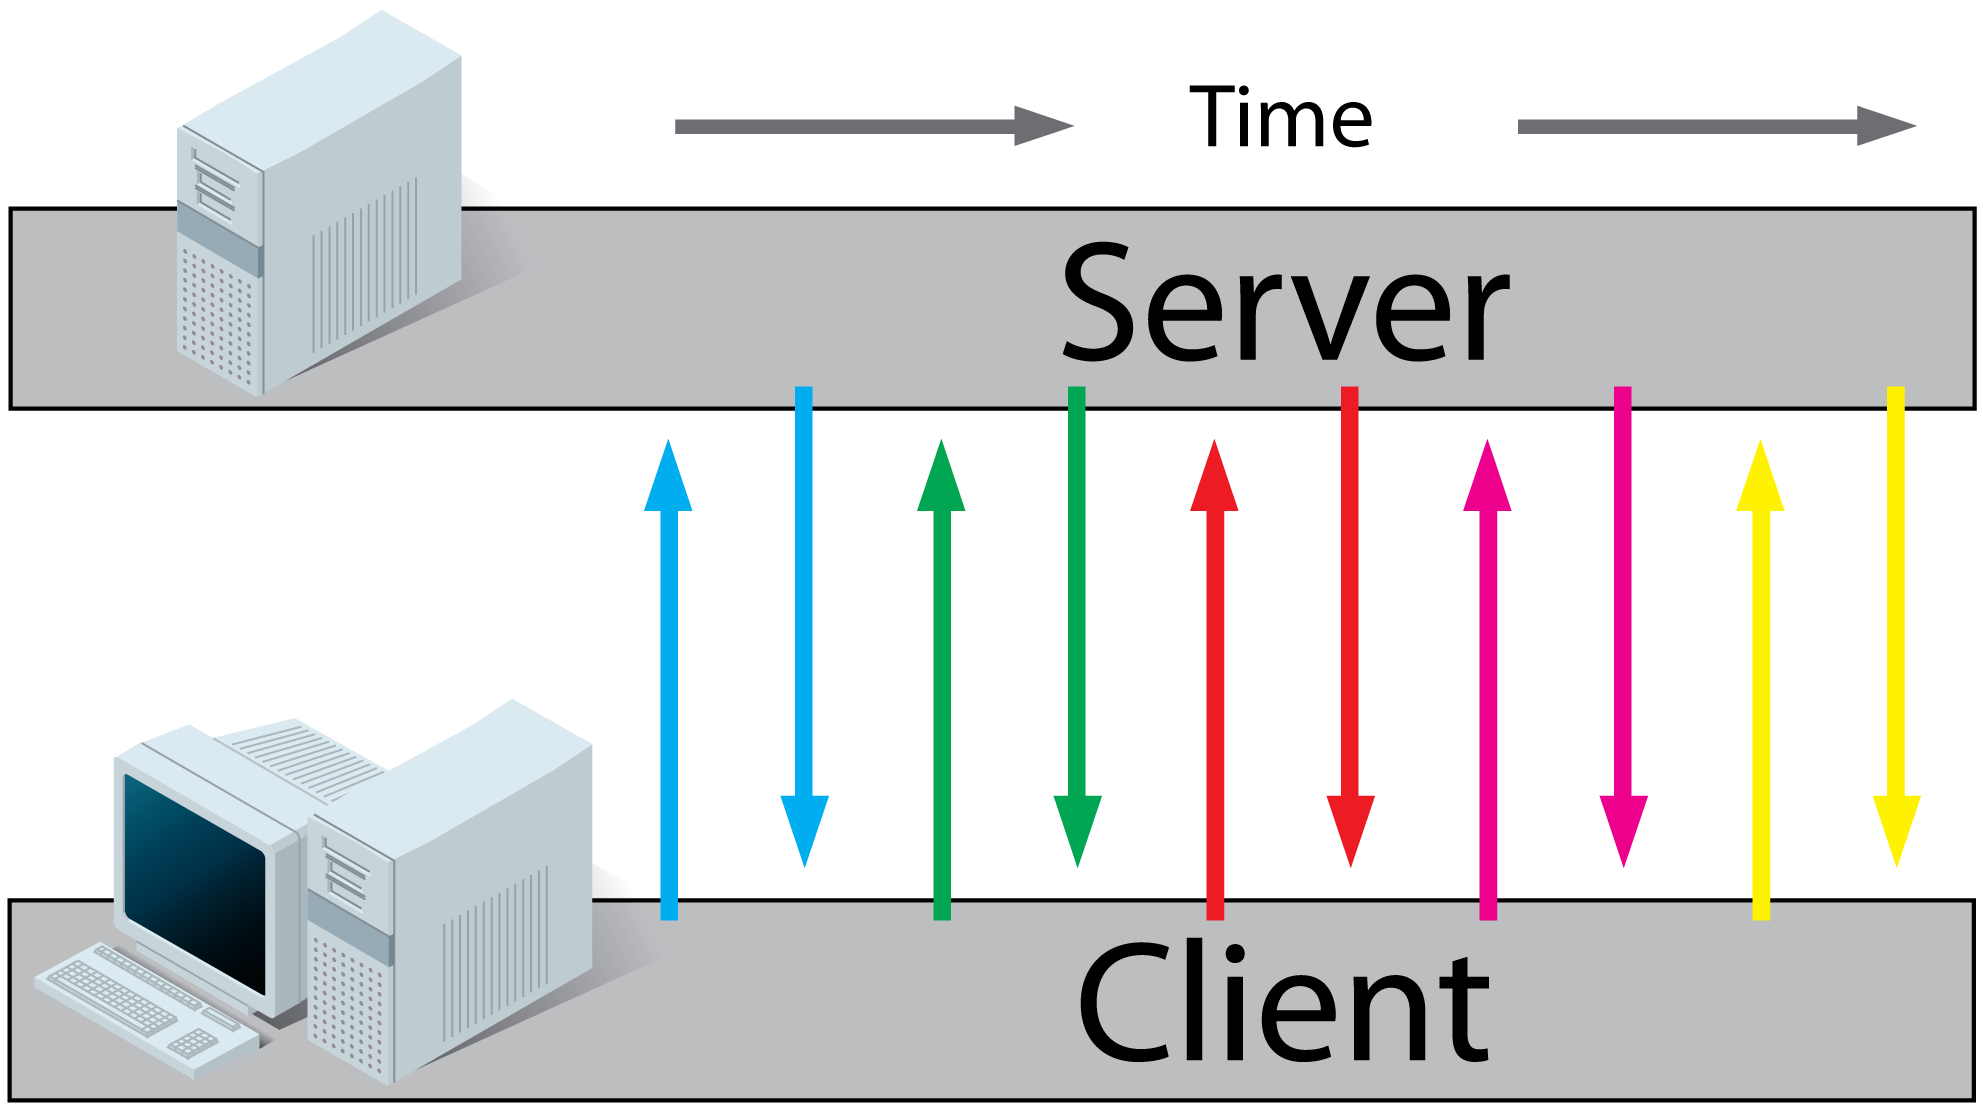
\includegraphics[scale=0.4]{Immagini/ajax_polling.png}
\end{figure}
\subsection{Long Polling Ajax}
\begin{enumerate}
	\item Il client richiede una pagina web al server usando il normale HTTP.
	\item Il client riceve la pagina web richiesta ed esegue il codice JavaScript contenuto nella pagina, il quale richiede un file al server.
	\item Il server non risponde immediatamente con l'informazione richiesta, ma aspetta finché non c'è una nuova informazione disponibile.
	\item Quando l'informazione è disponibile, il server risponde con questa.
	\item Il client riceve la nuova informazione e manda immediatamente un'altra richiesta al server, riavviando il processo.
\end{enumerate}
\begin{figure}[h]
	\centering
	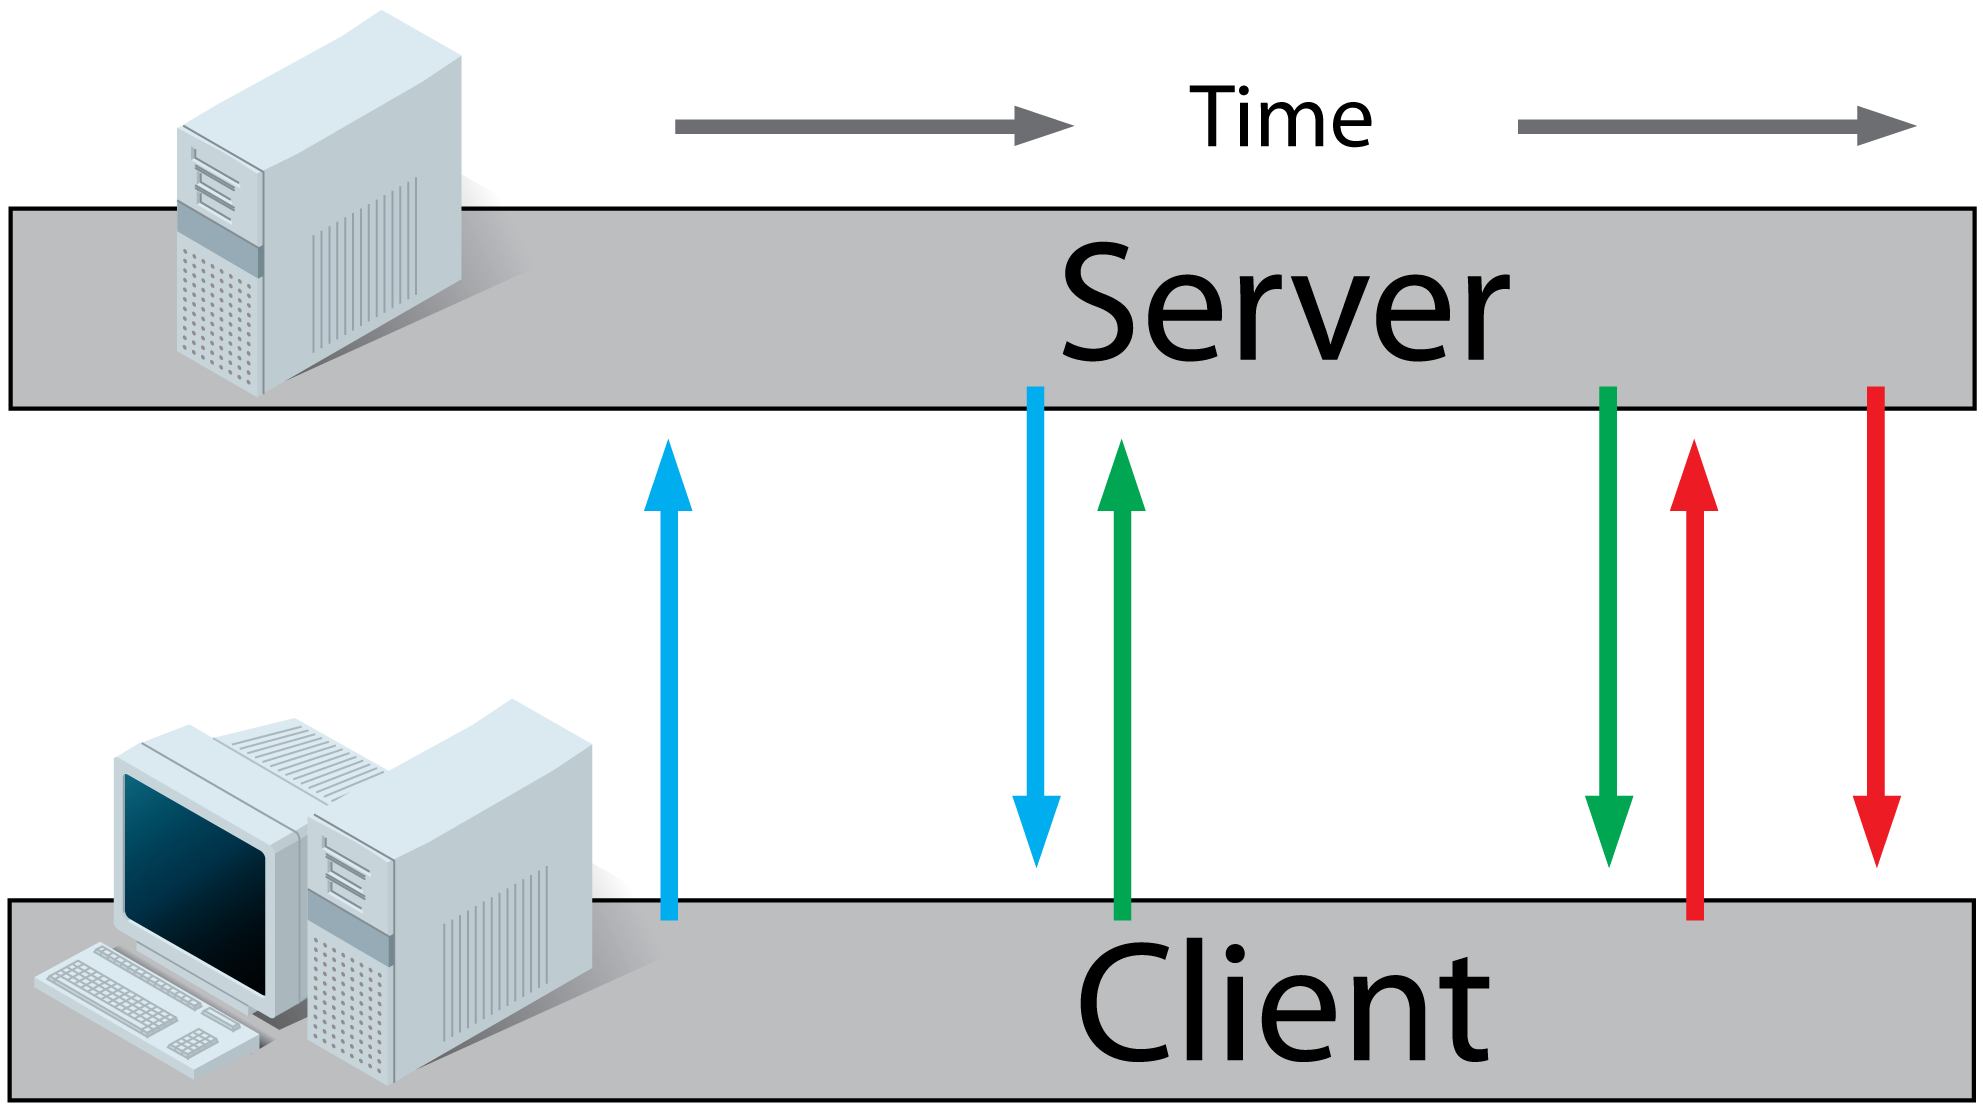
\includegraphics[scale=0.4]{Immagini/ajax_long_polling.png}
\end{figure}
\subsection{HTML5 Server Sent Events (SSE)}
\begin{enumerate}
	\item Il client richiede una pagina web al server usando il normale HTTP.
	\item Il client riceve la pagina web richiesta ed esegue il codice JavaScript contenuto nella pagina, il quale apre una connessione al server.
	\item Il server invia un evento al client non appena è disponibile una nuova informazione.
\end{enumerate}
\begin{figure}[h]
	\centering
	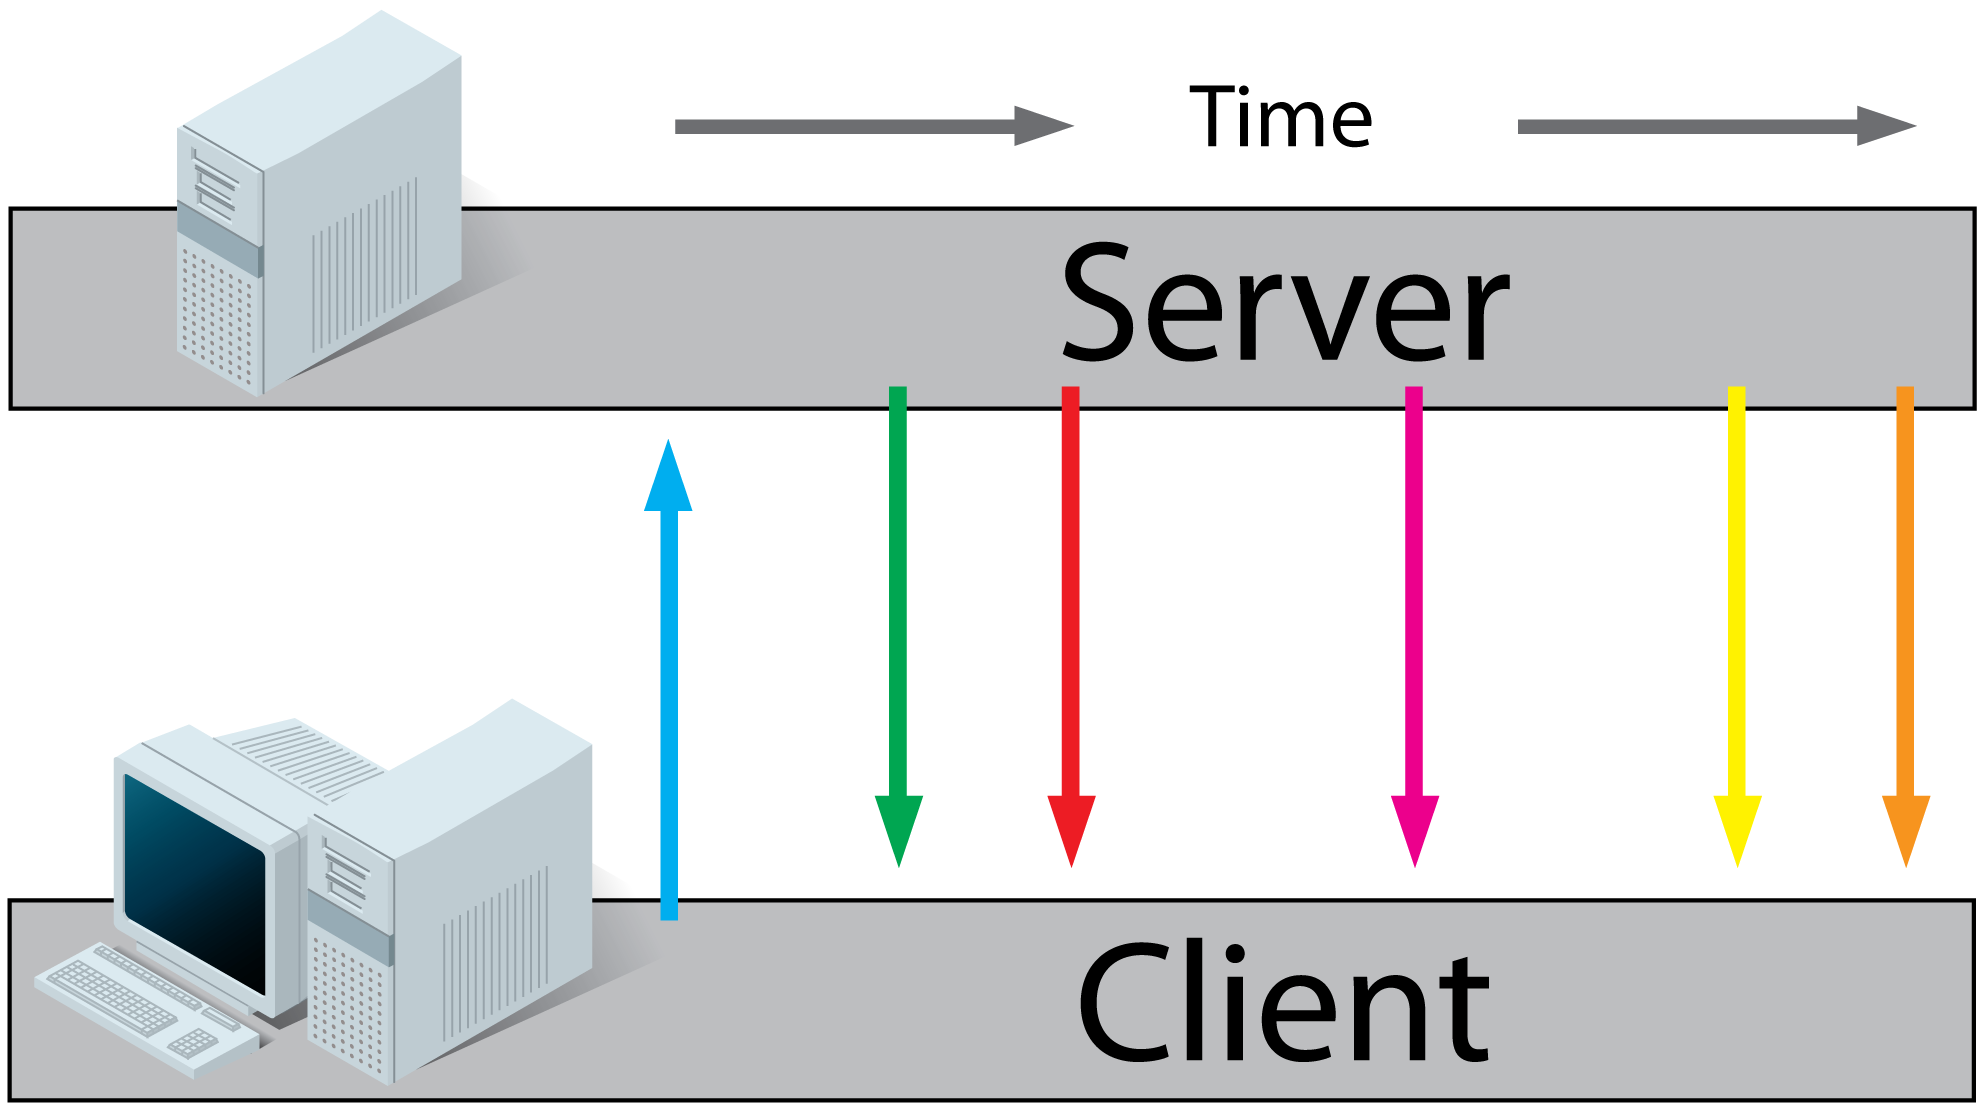
\includegraphics[scale=0.4]{Immagini/server_sent_events.png}
\end{figure}
\newpage
\subsection{HTML5 Websockets}
\begin{enumerate}
	\item Il client richiede una pagina web al server usando il normale HTTP.
	\item Il client riceve la pagina web richiesta ed esegue il codice JavaScript contenuto nella pagina, il quale apre una connessione al server.
	\item Il client e il server possono ora scambiarsi messaggi quando sono disponibili nuove informazioni (da qualsiasi lato).
\end{enumerate}
\begin{figure}[h]
	\centering
	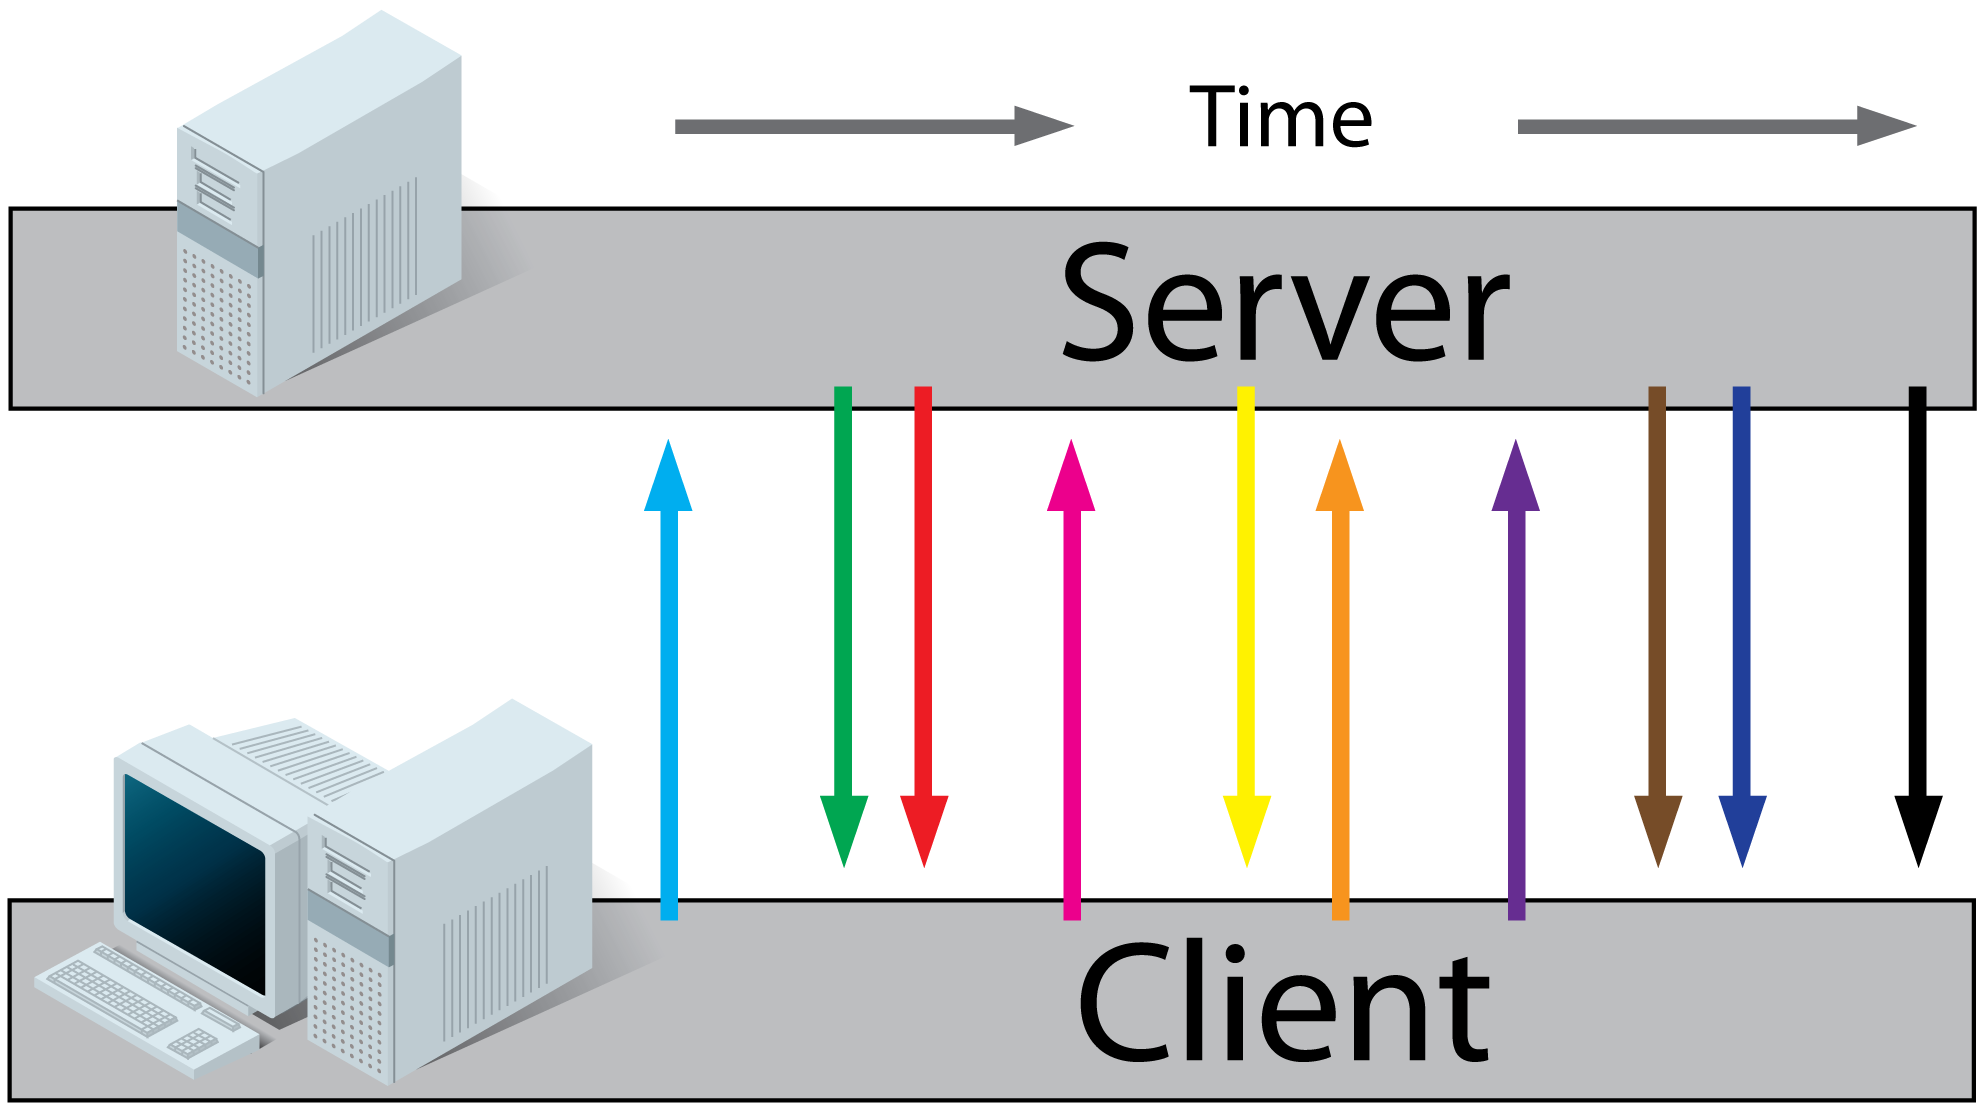
\includegraphics[scale=0.4]{Immagini/websockets.png}
\end{figure}